\documentclass[11pt]{amsart}

\usepackage{lmodern}
\usepackage[T1]{fontenc}
\usepackage{amsmath,amssymb,amsthm}
\usepackage{tikz}
\usepackage[margin=1in]{geometry}
\usepackage{microtype}
\usepackage[hidelinks]{hyperref}

\theoremstyle{plain}
\newtheorem{theorem}{Theorem}[section]
\newtheorem{proposition}[theorem]{Proposition}
\newtheorem{corollary}[theorem]{Corollary}
\theoremstyle{definition}
\newtheorem{definition}[theorem]{Definition}
\newtheorem{remark}[theorem]{Remark}

\newcommand{\code}[1]{\texttt{#1}}
\newcommand{\N}{\mathbb{N}}

\setlength{\emergencystretch}{3em}

\begin{document}

\title{A Complete Formal Verification of the Intel 4004}
\author{Charles C. Norton}
\date{July 2026}
\subjclass[2020]{Primary 68V20, 68V15; Secondary 68N30, 94C10}
\keywords{Intel 4004, formal verification, interactive theorem proving, Rocq, Coq, dependent types, instruction set architecture, differential testing, transistor netlist}

\begin{abstract}
The Intel 4004, shipped in 1971, was the first microprocessor: a complete four-bit central processing unit on one chip of roughly twenty-three hundred transistors, with forty-six instructions and its own family of memory and interface chips. Its smallness, once its defining constraint, now makes it one of the few processors that can be captured whole in a form a proof assistant can check. We present a complete formalization of the 4004 and its MCS-4 support chips in the Rocq prover: all forty-six instructions, the full system state, and the memory and input/output behavior, built over dependent fixed-width words that make the machine's legality true by construction rather than by hypothesis. We prove that the instruction decoder and encoder are exact inverses, that every instruction preserves the machine's structural invariant with no side conditions, and that a compiler for a small language with loops and conditionals emits read-only-memory images that provably compute the right result on the fetch-decode-execute machine. The entire development is axiom-free: \code{Print Assumptions} reports one hundred forty-eight machine-checked results, each closed under the bare type theory. We then confront the model with the chip itself, along a ladder of three independent references ending at a switch-level simulation of the transistor netlist recovered from Intel's own fabrication masks. The netlist agrees with the model on roughly eighty-six thousand observed bus values across fourteen test programs, and in the course of reaching that agreement it exposed and corrected a genuine error in the model, a mistaken value left in the address ring on a subroutine return past the stack's depth, a case the 1971 data sheet does not specify and every data-sheet-derived check had therefore inherited. The development is publicly available and machine-checked.
\end{abstract}

\maketitle

\section{Introduction}

In November 1971 Intel shipped a chip the size of a fingernail that held an entire central processing unit. The 4004 carried roughly twenty-three hundred transistors, worked in four-bit words, understood forty-six instructions, and ran on a clock of a few hundred kilohertz. It had been designed by Federico Faggin, from an architecture by Ted Hoff and Stanley Mazor, for a Japanese calculator, and it was the first microprocessor: the first time a general-purpose processor had been reduced to a single integrated circuit that anyone could buy. Everything that followed, the microcomputer and the personal computer and the processor in every phone, begins here.

The 4004 was small because it had to be, and that smallness is now an opportunity. Modern processors are far beyond the reach of a complete formal treatment; one verifies a component, a protocol, a pipeline stage, never the whole machine down to the last instruction. The 4004 is different. Its state fits on a page. Its instruction set fits in a table. A patient reader can hold the entire processor in mind at once, which means that a proof assistant can hold it too. This paper takes that possibility seriously and carries it through: a complete model of the 4004, every instruction and every register and the memory and interface chips around it, expressed as mathematics and checked, in full, by machine.

By ``checked by machine'' we mean something exact. The processor becomes a total function on a datatype of machine states, written in the Rocq prover (the system formerly called Coq). Every claim we make about it, that the decoder inverts the encoder, that no instruction can corrupt the machine's structure, that a compiled program computes what its source says, is a theorem in Rocq's logic, proved and mechanically verified, with the proof scripts available for anyone to re-run. There is no informal step and no appeal to authority. Moreover, because the 4004 is a finite discrete object with no real numbers or limits anywhere in sight, the development needs no axioms at all: \code{Print Assumptions}, the command that reports what a Rocq theorem depends on, returns for every one of our results the same verdict, closed under the global context, meaning the theorem rests on nothing but the bare type theory.

A proof about a model, however, is only ever a proof about the model. It certifies that our definitions have the properties we claim; it cannot certify that our definitions are the 4004. That second question, whether the mathematics matches the silicon, cannot be settled by proving more, only by confronting the model with the chip. We do this along a ladder of three independent references. The first is a second implementation of the instruction set, written in a different style directly from Intel's 1973 programming manual, against which we run millions of differential tests. The second is a third-party emulator, written by someone else for another purpose, which catches the errors a single author's two implementations might share. The third, and the one that matters most, is the chip itself. For the machine's thirty-fifth anniversary Intel released the 4004's schematics and the artwork of its fabrication masks, and from those masks a transistor-level netlist was recovered and checked. We drive a switch-level simulation of that netlist through the memory-bus protocol and compare it, cycle by cycle, with our model. Across fourteen test programs and roughly eighty-six thousand observed values on the pins, the transistors and the model agree.

They did not agree at first, and the disagreement is the most instructive result in the paper. The 4004 keeps its return addresses in a small ring of registers, three deep, and no document of 1971 says what happens if a program returns from a subroutine it never called, walking the ring past its depth. Our model, following the natural reading of the data sheet, resumed a stale entry unchanged. The transistors did something slightly different: the vacated entry had been incremented during the returning instruction's own fetch and was abandoned without being written back, so the recovered address is one greater than the model produced. This is exactly the kind of detail a data sheet omits, which is why it had slipped past not only the proofs but also the independent reference and the emulator: all three descend from the same human reading of the same silent manual. The masks descend from the silicon. They caught the error, we corrected the model, and the corrected model now matches.

We should be careful about what is new here, because processors have been verified before. Beginning in the 1980s a line of work verified processor \emph{designs}: one specifies a machine in a logic or a hardware description language and proves the specification has the properties one wants, as in Hunt's FM8501 and FM9001 \cite{hunt} and the stack of verified components built around them. That is a different activity from ours, and a complementary one. We do not verify a design of our own; we build a faithful mathematical model of a specific historic commercial processor and tie it to the physical artifact, the actual transistors on the actual die, recovered from the actual masks. To our knowledge no formal treatment of the 4004 reaches this completeness, and the grounding of an instruction-set model in a chip's own fabrication masks, rather than in a design one has written oneself, is unusual for processor verification generally. Our contributions are three.

\begin{enumerate}
\item \textbf{A complete axiom-free model of the 4004 and MCS-4.} All forty-six instructions, the full nineteen-field system state, the memory hierarchy of the 4002 RAM and the ports of the 4001 ROM, and the fetch-decode-execute machine over them, built on dependent fixed-width words so that a value out of range is not a value the type admits (Sections~\ref{sec:machine} and~\ref{sec:math}). The machine's legality is true by construction, and its structural invariant is preserved by every instruction with no side condition.

\item \textbf{Proofs of correctness, machine-checked.} The decoder and encoder are exact inverses on well-formed instructions; every instruction preserves the invariant unconditionally; a Hoare logic covers all forty-six instructions; and a compiler for a small imperative language with loops and conditionals emits read-only-memory images that provably run on the machine to the intended result (Section~\ref{sec:proofs}). The development is axiom-free (Section~\ref{sec:rocq}).

\item \textbf{Validation against the silicon.} Three independent references, ending at a switch-level simulation of the transistor netlist taken from Intel's masks, agree with the model across roughly eighty-six thousand observed bus values; the netlist comparison found and corrected a genuine error in the model (Section~\ref{sec:validation}).
\end{enumerate}

The remainder of the paper is a guided tour of the machine and its verification. Section~\ref{sec:machine} introduces the 4004 itself, in enough concrete detail that the rest is legible. Section~\ref{sec:math} turns the machine into mathematics and states the structural theorems. Section~\ref{sec:proofs} describes what the model proves above the instruction level. Section~\ref{sec:validation} climbs the validation ladder to the transistors. Section~\ref{sec:rocq} reports the Rocq development and its axiom footprint, and Section~\ref{sec:outlook} closes with the one question the masks cannot answer.

\section{The machine}\label{sec:machine}

To read the rest of the paper one needs to know the 4004 as its programmer did, so we describe it plainly before formalizing it. The processor works in \emph{nibbles}, four-bit quantities holding a value from zero to fifteen, and in \emph{bytes} of eight bits. It has a four-bit accumulator, the register where arithmetic happens, and a single carry bit beside it. It has sixteen general index registers, each a nibble, which the instruction set also treats as eight register \emph{pairs} when it needs a byte. Program memory is separate from data memory, as on a Harvard machine: instructions live in read-only memory addressed by a twelve-bit program counter, giving an address space of four thousand ninety-six bytes, organized as sixteen pages of two hundred fifty-six.

Subroutine calls are supported by a small hardware stack. The program counter and three saved return addresses live together in a ring of four twelve-bit registers with a pointer selecting which one is currently the program counter. A call rotates a return address into the ring and advances the pointer; a return rotates it back. Because the ring is only four deep, a fourth nested call overwrites the oldest saved address, and the depth of subroutine nesting is genuinely three. This ring, small as it is, is where the subtlest behavior of the machine lives, and we will return to it.

Around the processor sit the other members of the MCS-4 family. The 4001 is a read-only-memory chip that also carries a four-bit input/output port; up to sixteen of them supply the full program address space, and their ports give the processor its outside world. The 4002 is a random-access memory chip with an unusual internal organization: it holds four registers, each of twenty four-bit characters, sixteen of them ``main memory'' and four of them ``status,'' and it too carries an output port. Data memory is addressed hierarchically. An instruction called \code{DCL} selects a bank of RAM chips by driving command lines; an instruction called \code{SRC} then sends a chip, register, and character address; and read and write instructions move a single nibble at the selected place. The model represents the whole hierarchy, four banks of four chips of four registers of twenty characters, exactly as the chips are wired.

The instruction set has forty-six members, each one or two bytes long. There are the expected arithmetic and logic operations on the accumulator (add, subtract, increment, rotate, complement, and a decimal-adjust for binary-coded-decimal arithmetic); loads and exchanges between the accumulator and the index registers; the control-flow instructions (unconditional jump, jump to subroutine, return, conditional jump on the accumulator or carry or an external test pin, and an increment-and-skip that builds counting loops); and the memory and port instructions that reach the 4001 and 4002 chips. One instruction, \code{WPM}, even writes program memory through external programming hardware, which is how a 4004 system could modify its own code. Timing is simple and fixed: a machine cycle is eight clock periods, a one-byte instruction takes one machine cycle and a two-byte instruction takes two, and there is no pipeline and no wait state, so the time a program takes is exactly the sum of its instructions' cycle counts.

That is the entire machine. Every sentence above becomes a definition in what follows.

\section{The machine as mathematics}\label{sec:math}

\subsection{Bounds by construction}

The first design decision is the one that governs everything after it, and it concerns how to represent a four-bit quantity. The obvious choice is to use ordinary natural numbers and carry, everywhere, the side condition that a nibble is less than sixteen. This works, but it is miserable: every register, every memory character, every intermediate result drags a hypothesis $v < 16$ through every proof, and the invariant of the whole machine becomes a long conjunction of range conditions that each instruction must be shown to maintain. We take the other road. A four-bit word is not a natural number that happens to be small; it is an inhabitant of a type whose every element is small.

\begin{definition}[the type of $w$-bit words, \code{word}]\label{def:word}
For a width $w$, a $w$-bit word is a natural number paired with a proof that it fits:
\[
  \code{word } w \;:=\; \{\, n : \N \mid (n <_? 2^w) = \code{true} \,\}.
\]
The nibble, byte, and twelve-bit address types are \code{word 4}, \code{word 8}, and \code{word 12}; the accessor \code{wval} returns the underlying value.
\end{definition}

The fitting condition is written as a \emph{boolean} test $n <_? 2^w$ equated to \code{true}, and this small choice has a large consequence. Booleans have decidable equality, and a type with decidable equality has unique identity proofs, a theorem of the bare type theory that needs no axiom. So two words are equal as soon as their values are equal: the proofs they carry cannot differ in any way that matters (\code{word\_eq}). One may therefore compute with words as freely as with plain numbers, comparing and rewriting them by their values alone, while the type quietly guarantees that no nibble ever reaches sixteen. The constructor that builds a word from an arbitrary number reduces it modulo $2^w$ and attaches a canonical proof, arranged so that equalities between concrete machine states reduce to \code{true} under Rocq's evaluator (\code{mkw}, with the canonicalizer \code{bcanon}); and when the development is extracted to executable OCaml, the proof is erased entirely and a word becomes a bare machine integer, so nothing of this apparatus survives into the running code.

The payoff appears immediately at the level of the whole machine. Because every quantity is bounded by its type, the invariant that says ``this is a legal 4004 state'' no longer needs to mention a single numeric range. It needs only to fix the sizes of the containers.

\begin{definition}[well-formed state, \code{WF}]\label{def:wf}
A state is well-formed when its lists have the right lengths: sixteen index registers; a RAM system of four banks, each of four chips, each of four registers, each of twenty characters; sixteen entries in each of the two port arrays and in the port-direction array; and four thousand ninety-six bytes of program memory. These seven length conditions are the entire predicate.
\end{definition}

Seven structural facts, and not one value bound, because the values cannot be out of bounds. This is the concrete reward of Definition~\ref{def:word}, and it makes the central preservation theorem, below, almost mechanical to prove.

\subsection{State, decoding, and execution}

The machine's state is a record of nineteen fields, each now typed by the quantity it holds: the accumulator (a nibble), the index registers (a list of nibbles), the carry (a boolean), the four rows of the address ring (twelve-bit words), the RAM system, the command-line latch set by \code{DCL}, the address latched by \code{SRC}, the ROM output-port latches and input pins and their mask-programmed directions, program memory, the external test pin, and the three registers of the program-memory writer. The address ring deserves a word on representation, because its encoding is what later lets a single theorem capture the subroutine mechanism. Rather than store a rotating hardware pointer, the state keeps the four rows in pointer-relative coordinates, the current program counter and the three saved rows in order behind it, so that a call and a return become fixed rotations of four fields (Figure~\ref{fig:ring}). We prove this representation equivalent to an explicit model with a numeric pointer (\code{ring\_matches}, \code{rotating\_ring\_complete}), so nothing is lost by the convenient choice.

\begin{figure}[ht]
\centering
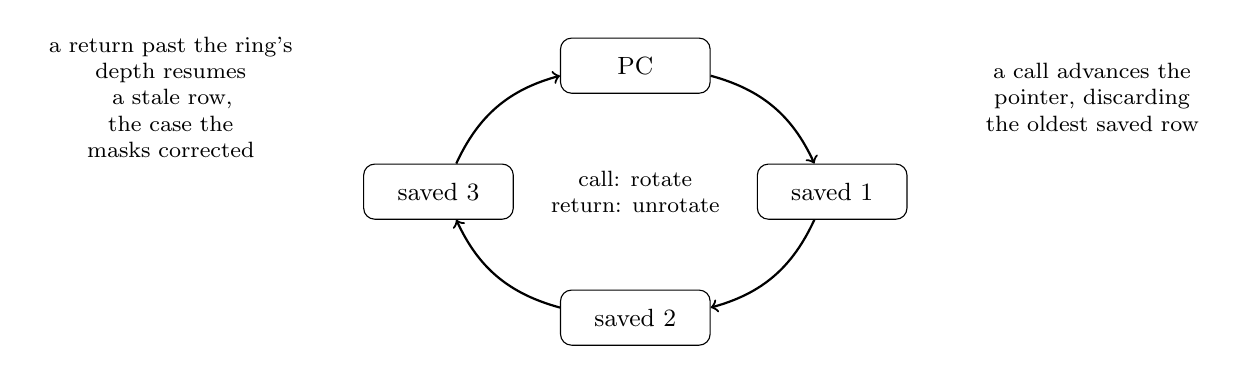
\begin{tikzpicture}[scale=1.0]
  \tikzset{row/.style={draw, rounded corners, minimum width=1.9cm, minimum height=0.7cm, font=\small}}
  \node[row] (pc)  at (0, 1.6)  {PC};
  \node[row] (s1)  at (2.5, 0)  {saved 1};
  \node[row] (s2)  at (0, -1.6) {saved 2};
  \node[row] (s3)  at (-2.5, 0) {saved 3};
  \draw[->, thick] (pc) to[bend left=25] (s1);
  \draw[->, thick] (s1) to[bend left=25] (s2);
  \draw[->, thick] (s2) to[bend left=25] (s3);
  \draw[->, thick] (s3) to[bend left=25] (pc);
  \node[font=\footnotesize, align=center] at (0,0) {call: rotate\\return: unrotate};
  \node[font=\footnotesize, align=center, text width=3.2cm] at (5.8, 1.2)
    {a call advances the\\pointer, discarding\\the oldest saved row};
  \node[font=\footnotesize, align=center, text width=3.4cm] at (-5.9, 1.2)
    {a return past the ring's\\depth resumes a stale row,\\the case the masks corrected};
\end{tikzpicture}
\caption{The 4004 address register as a ring of four twelve-bit rows: the program counter and three saved return addresses. A call rotates one way and a return the other. The behavior on a return past the third saved row is unspecified by the 1971 data sheet, and is where the transistor netlist corrected the model (Section~\ref{sec:validation}).}\label{fig:ring}
\end{figure}

An instruction is one of forty-six constructors of an inductive type, its operands already typed by their widths, so that, for example, a jump carries a genuine twelve-bit address and a load-immediate carries a genuine nibble. Turning bytes into instructions is a total function.

\begin{definition}[decoding, \code{decode}]\label{def:decode}
\code{decode} maps a pair of bytes to an instruction, reading the top four bits of the first byte as an operation and the rest as operands, and returning the no-op for the byte patterns Intel left unused. It is total: every one of the sixty-five thousand five hundred thirty-six byte pairs decodes to something.
\end{definition}

Encoding runs the other way, and the two are inverse wherever the instruction is meaningful. The only well-formedness an instruction needs is a parity condition on the register-pair instructions, since operand widths are already guaranteed by their types; there are no other side conditions to carry.

\begin{theorem}[the decoder inverts the encoder, \code{decode\_encode\_id}]\label{thm:bijection}
For every well-formed instruction $i$, decoding the bytes that encode $i$ returns $i$. Conversely, re-encoding a decoded byte pair yields bytes that decode to the same instruction, and every well-formed instruction is the decoding of some byte pair (\code{decode\_surjective\_on\_wf}).
\end{theorem}

This is the sense in which the assembler and disassembler agree: no instruction is lost or altered by a round trip through its binary form. The proof is a case analysis over the instruction constructors with the arithmetic of the encoding, and because the operands are typed, the arithmetic never has to reason about out-of-range fields.

Execution is the heart of the model: a total function that takes a state and an instruction and returns the next state.

\begin{definition}[execution, \code{execute}]\label{def:execute}
\code{execute} sends a state and an instruction to the successor state, defined case by case over the forty-six instructions. Each case constructs the next state through field updates, leaving every unmentioned field alone.
\end{definition}

We insist that \code{execute} be faithful, not simplified, and this is a real commitment rather than a slogan. Where a naive model would idealize the hardware, ours follows it. A memory-bank selection that drives several command lines at once writes every selected bank, not a nominal one. A subroutine call and return are the ring rotations of Figure~\ref{fig:ring}, including the overwrite of the oldest row on a fourth call. The program-memory write assembles a byte from two four-bit transfers through an external latch pair, exactly as the 4008/4009 programming chips do, rather than writing a byte at a stroke. The output ports are mask-configured as inputs or outputs, and a read returns the driven pins or the latched value according to that configuration. These are the behaviors that make the difference between a model of the 4004 and a model of a 4004-like machine, and putting them into \code{execute} directly, rather than into a separate ``realistic'' layer, is what lets us state and prove properties about the machine the hardware actually is.

With the invariant reduced to lengths and the values bounded by their types, the property one most wants of \code{execute} costs almost nothing to state and holds without qualification.

\begin{theorem}[execution preserves well-formedness, \code{execute\_preserves\_WF}]\label{thm:preserve}
For every state $s$ and instruction $i$, if $s$ is well-formed then so is \code{execute} $s\ i$. No hypothesis on the instruction is required.
\end{theorem}

Compare this with what the same theorem would demand under the naive representation, where every case would have to re-establish that every touched value is still in range. Here the type system has already discharged all of that, and the proof reduces to checking that the field updates preserve the container lengths, which they do uniformly. The fetch-decode-execute machine is then the obvious composition, reading the instruction at the program counter from memory and executing it (\code{step}, and its iterate \code{steps}), and well-formedness is preserved along any run (\code{steps\_preserve\_WF}). Two immediate corollaries record that the machine can never wander out of memory or corrupt it: the program counter always stays within the twelve-bit space (\code{no\_arbitrary\_jumps}), and every byte of program memory remains a byte (\code{memory\_safety}).

\section{What the model proves}\label{sec:proofs}

A faithful executable model is worth having on its own, but the point of building it in a proof assistant is to reason above the level of single instructions, and the development does so in three directions.

\subsection{A program logic for the instruction set}

The first is a Hoare logic, the standard calculus of preconditions and postconditions, instantiated for the 4004. A triple asserts that if a state satisfies its precondition and is well-formed, then after an instruction it satisfies its postcondition and is still well-formed, so the invariant rides along for free. Every one of the forty-six instructions has a rule (the arithmetic and logic instructions are covered uniformly by a single rule whose postcondition is the data-sheet reference function, and the rest individually), together with the structural rules of consequence, conjunction, and framing that let one reason about the registers, the accumulator, and memory independently when an instruction touches only some of them. On top of the per-instruction rules sits a program-level logic with a sound weakest-precondition calculus (\code{wp\_soundness}, \code{vc\_sound}), and a handful of verified example programs, among them a decimal addition routine proved correct against ordinary base-ten arithmetic (\code{bcd\_add\_prog\_correct}) and separation-logic reasoning over the RAM hierarchy so that a write to one cell provably leaves the rest untouched (\code{wrm\_sep\_frame}).

\subsection{A verified compiler}

The second direction is the one a reader may find most vivid, because it closes the loop from a source program all the way to the running silicon-faithful machine. We define a small imperative language with assignment, sequencing, conditionals, and while loops over the index registers, give it a straightforward meaning as a function on register environments, and write a compiler from it to 4004 machine code. The compiler is not a toy that ignores the machine's awkwardness; it handles the real constraint that the 4004's conditional jump can only reach within a two-hundred-fifty-six-byte page, by emitting a short page-local skip over an absolute jump and padding across page boundaries where needed, so that compiled programs may span pages and sit anywhere in memory. The correctness theorem states that this all works end to end.

\begin{theorem}[compiled programs run correctly, \code{compiled\_cstmt\_runs\_on\_machine}]\label{thm:compiler}
For a well-formed source statement, assembling the compiler's output into a program-memory image, starting the machine at address zero, and running the fetch-decode-execute loop leaves the index registers holding exactly the values the source language's semantics prescribes, whenever that semantics terminates.
\end{theorem}

The theorem is about the real machine, not an idealization of it: the same \code{step} function of Section~\ref{sec:math}, reading the same bytes the compiler emitted from the same memory, decoding and executing them one by one. Underneath the compiler's correctness is a general simulation principle for control-flow graphs held in memory (\code{pc\_indexed\_simulation}), which is also what verifies a hand-written counting loop running on the machine for its exact number of iterations.

\subsection{Timing and machine cycles}

The third direction is time. The 4004's timing is fixed and knowable, and the model makes it a theorem rather than a comment. Each instruction has a cycle count, straight-line code takes exactly the sum of its counts with no pipeline effects to spoil the arithmetic (\code{machine\_time\_straightline}), and a concrete counting loop is proved to take its exact number of clock periods (\code{iszloop\_machine\_time}, two hundred seventy-two of them). Below the instruction level, a finer model executes each instruction as its sequence of machine cycles and is proved to refine the instruction-level machine (\code{microcycle\_refines\_steps}), which is the granularity at which the machine speaks to the outside world, and therefore the granularity at which we will compare it with the transistors.

\section{Checking the model against the chip}\label{sec:validation}

Everything to this point is a theorem about our definitions. Whether those definitions are the 4004 is a different question, an empirical one, and we answer it by confronting the model with references it does not share an origin with. The principle is triangulation: a single author's model can be self-consistent and wrong in a way that self-consistency will never reveal, so one seeks witnesses that fail independently. We use three, of increasing authority.

\subsection{An independent reference}

The first witness is a second implementation of the instruction set, written in OCaml directly from Intel's 1973 programming manual, deliberately in a different style from the model, and used as a differential oracle. We extract our verified model to executable OCaml and run the two side by side over enormous input sets: the decoding of all sixty-five thousand five hundred thirty-six byte pairs, the arithmetic and logic unit over every accumulator, carry, and operand combination, the program-counter behavior of every conditional jump over all four thousand ninety-six addresses and all sixteen conditions, the subroutine ring including its overflow and underflow, the RAM across its whole address space, and the timing of every instruction. This is several million checks, and it catches the errors of transcription and arithmetic that are easy to make and hard to see by inspection. It does not catch errors of understanding, because both implementations are ours and read the same manual.

\subsection{A third-party emulator}

The second witness addresses exactly that gap. Pyntel4004 \cite{pyntel} is an emulator of the 4004 written independently, by another author, for another purpose. We replay our model's exhaustive arithmetic vectors through it and compare. Most operations agree on every input; the disagreements are illuminating, because they turn out to be defects in the emulator rather than in the model, and we adjudicate each against the data sheet: its addition reduces an overflowing sum by fourteen instead of sixteen, its decrement writes a constant, its conditional jump mishandles the inversion bit and the page composition of its target, and it does not wrap the twelve-bit address space. That a careful independent emulator carries this many defects is itself a small lesson in how easily a 4004 can be modeled almost right, and the cross-check is only meaningful because the disagreements can be traced to a shared authority, the data sheet, that declares which side is correct. But that is also the limitation of the first two witnesses together: both they and the model ultimately rest on the same documents, and where the documents are silent, all three can be wrong in the same way.

\subsection{The transistors}

The third witness rests on nothing but the silicon. For the 4004's thirty-fifth anniversary Intel released the chip's schematics and the artwork of its fabrication masks under a non-commercial license \cite{masks}. From that artwork Lajos Kintli recovered a transistor-level netlist, extracting the devices from the mask layers and machine-comparing them against a netlist independently recognized from the redrawn schematic until the two agreed, roughly eighteen hundred transistors and four hundred pull-up resistors, and validated the result by simulating MCS-4 programs on it \cite{kintli}; the netlist is redistributed in a form we pin by content \cite{monta}. We wrote an independent switch-level simulator for that netlist, one that knows nothing of our model, resolving the state of every node from the conducting transistors the way the physical circuit does, and drove it through the memory-bus protocol with a full four-thousand-ninety-six-byte memory. What the simulated chip puts on its pins, the fetch addresses it emits and the data it drives and the command lines it raises, is exactly what an oscilloscope on a real 4004 would see, so the comparison is against the physical behavior of the device and not against any description of it.

We compare the transistors with the model cycle by cycle across fourteen test programs: the undefined opcodes, the full arithmetic and logic unit, the register file, conditional branching under every condition with the test pin driven both ways, the loop and indirect-addressing instructions, the page-boundary and address-wrap cases, the subroutine ring pushed and popped past its depth, memory-bank selection over every command-line code, and seeded pseudo-random straight-line programs. Across roughly eighty-six thousand observed values on the pins, the netlist and the model agree on every one.

They did not at first, and the single disagreement is worth telling in full, because it is precisely the failure the three-witness ladder was built to catch. On the fourth consecutive return from a subroutine, a return past the ring's depth, the model and the transistors produced different addresses. The 1971 data sheet does not define this case, and our model had taken the natural reading, that the return resumes the stale row as it stands. The transistors showed otherwise. During the returning instruction's own fetch the row is incremented, as every fetched address is, and the ring rotation then abandons that row without writing the increment back, so the address the hardware resumes is one greater than the model's. It is a difference of one, in a case a program should never reach, and it had survived everything: the hundred forty-eight machine-checked theorems, the several million differential checks against the independent reference, and the entire emulator cross-check, because every one of those rests on the data sheet, and the data sheet is silent here. Only the masks, which rest on the silicon, disagreed, and they were right. We corrected the model's return to leave the incremented value in the abandoned row (\code{ring\_pop}), reproved the ring theorems and the isomorphism of Section~\ref{sec:math} against the corrected definition, and reran the ladder; the corrected model matches the transistors on all fourteen programs.

\section{The development in Rocq}\label{sec:rocq}

The development \cite{repo} is carried out in Rocq~9 over its standard library. The model and its proofs are distributed over five theory files: the machine itself, its state, decoding, execution, and the preservation theorems (\code{machine.v}); the behavioral theory, including the arithmetic correctness, the address ring and its isomorphism, the timing model, and the microcycle refinement (\code{behavior.v}); the Hoare and separation logic and the verified straight-line compiler (\code{verification.v}); the control-flow simulation and the compiler for conditionals and loops (\code{control.v}); and the fidelity theorems that pin down the underspecified and boundary behaviors (\code{fidelity.v}). A sixth file collects the headline results, extracts the model to OCaml for the differential harness, and prints the axiom footprint of each. The three validation layers live beside the theories: the OCaml differential reference, the Python cross-check against Pyntel4004, and the netlist harness with its switch-level simulator and its bus-level comparator.

The axiom footprint is empty. \code{Print Assumptions} on each of the one hundred forty-eight headline results reports the same verdict, closed under the global context, with no admitted proofs and no axioms of any kind, classical or otherwise. This is stronger than one can achieve for most formalized mathematics, and the reason is the subject matter: the 4004 is a finite discrete object, its every quantity a bounded natural number and its every operation a computation, so nothing in the development ever reaches for the real numbers or the classical principles their construction requires. The machine is small enough, and concrete enough, to stand on the bare type theory alone.

\section{A worked example}\label{sec:demo}

The compiler theorem of Section~\ref{sec:proofs} is easiest to believe when one watches it run, so we trace a single program the whole way from source to execution on the machine. Take a countdown loop in the small language, which sets an index register to three and decrements it to zero:
\begin{center}
\code{R0 := 3;\quad while R0 <> 0 do R0 := R0 - 1}
\end{center}
Its meaning is not in doubt, and the source semantics agrees that it leaves \code{R0} at zero (\code{cwhile\_demo\_sem}). Compiling it yields a seventeen-byte program-memory image, which the development produces explicitly rather than on faith:
\begin{center}
\code{D3 B0 A0 14 07 40 09 40 11 D1 B8 A0 F1 98 B0 40 02}
\end{center}
Every pair of hexadecimal digits is a real 4004 instruction. The first two load the constant three and move it into \code{R0}; the rest are the loop, which loads \code{R0}, tests it against zero with a conditional jump, and when it is not yet zero clears the carry, subtracts one, stores the result back, and jumps to the loop head. The one subtlety is that conditional jump, which on the 4004 can reach only within its own two-hundred-fifty-six-byte page, so the compiler has rendered the single source test as a short local skip over two absolute jumps, one into the loop body and one to the exit beyond it. This is the page handling of Section~\ref{sec:proofs} at work, and it is why three lines of source become seventeen bytes.

Now the payoff. Load those seventeen bytes into program memory at address zero, start the machine, and run the fetch-decode-execute loop of Section~\ref{sec:math}, the very same \code{steps} function that carries the correctness proofs. After thirty-five steps the program counter has reached the loop's exit and register \code{R0} holds zero, and this is a theorem, checked by evaluation inside Rocq over the same bytes the compiler emitted (\code{cwhile\_demo\_machine}). The source promised zero, the compiler produced those bytes, and the machine, executing them one instruction at a time, delivers zero. Theorem~\ref{thm:compiler} is that chain proved in general; this is one run of it, laid out in full.

\section{Outlook}\label{sec:outlook}

The model is complete at the level of the instruction set and validated against the transistors at the level of the pins, and two directions remain. One is a fully formal equivalence: our netlist comparison is differential, a cycle-by-cycle agreement over many programs rather than a proof, and a machine-checked equivalence between the transistor netlist and the instruction-level model would close the gap between overwhelming evidence and proof. That is a substantial undertaking, a verification in its own right, and it would rest on the differential agreement established here as its specification.

The other direction needs a bench rather than a proof. One behavior of the MCS-4 system is beyond even the masks: when a memory-bank selection drives several command lines at once and a program then reads, several RAM chips place their data on the shared bus simultaneously, and what results is an analog contention between chips that no digital netlist of the processor can settle. Our model gives this case a definite reading and marks it as a convention; confirming it, or correcting it as the masks corrected the subroutine ring, would take a physical 4004 and its memory chips wired on a bench and watched. It is a fitting place for the machine to have the last word. The first microprocessor can be captured whole in mathematics, proved correct without a single axiom, and matched against its own transistors down to the last pin, and there remains, still, one question that only the silicon itself can answer.

\begin{thebibliography}{99}
\raggedright

\bibitem{repo} C.~C. Norton, intel-4004-verified: a complete machine-checked formalization of the Intel 4004, \url{https://github.com/CharlesCNorton/intel-4004-verified} (2026).

\bibitem{mcs4} Intel Corporation, \emph{MCS-4 Micro Computer Set Users Manual} and \emph{MCS-4 Assembly Language Programming Manual}, Intel, 1973.

\bibitem{faggin} F.~Faggin, M.~E. Hoff, S.~Mazor, and M.~Shima, The history of the 4004, \emph{IEEE Micro} \textbf{16} (1996), no.~6, 10--20; see also F.~Faggin, The making of the first microprocessor, \emph{IEEE Solid-State Circuits Mag.} \textbf{1} (2009), no.~1, 8--21.

\bibitem{hunt} W.~A. Hunt, Jr., \emph{FM8501: A Verified Microprocessor}, Lecture Notes in Artificial Intelligence \textbf{795}, Springer, 1994; W.~A. Hunt, Jr. and B.~Brock, A formal HDL and its use in the FM9001 verification, \emph{Philos. Trans. Roy. Soc. London Ser.~A} \textbf{339} (1992), 35--47.

\bibitem{masks} Intel~4004 35th anniversary project: schematics and mask artwork of the MCS-4 family, released under a non-commercial license, \url{https://www.4004.com/} (2006--2009).

\bibitem{kintli} L.~Kintli, i400x analyzer: netlist and layout extraction and transistor-level simulation of the Intel MCS-4 family, \url{https://www.4004.com/} (2008--2018).

\bibitem{monta} P.~Monta, FPGA-netlist-tools: translating transistor netlists to hardware description languages, including the recovered 4004 layout netlist, \url{https://github.com/pmonta/FPGA-netlist-tools} (2011).

\bibitem{pyntel} Pyntel4004: an Intel 4004 emulator written in Python, \url{https://github.com/alshapton/Pyntel4004}.

\bibitem{rocq} The Rocq Development Team, \emph{The Rocq Prover} (formerly Coq), \url{https://rocq-prover.org} (2025).

\bibitem{leroy} X.~Leroy, Formal verification of a realistic compiler, \emph{Comm. ACM} \textbf{52} (2009), no.~7, 107--115.

\bibitem{sail} A.~Armstrong et al., ISA semantics for ARMv8-A, RISC-V, and CHERI-MIPS, \emph{Proc. ACM Program. Lang.} \textbf{3} (2019), POPL, article 71.

\end{thebibliography}

\end{document}
